% 
% EMSEC seminar template, 24.09.2010
% david.oswald@rub.de
% 
% based on
% EMSEC thesis template, 13.09.2010
% 
% Calls all chapters
% Each chapter is contained in a seperate "\input" file 
% Style: doublesided, scrreport, dina4
%
% Benedikt Driessen, 2010
% benedikt.driessen@rub.de
%

% *************************************************************
% ENTER INFORMATION ABOUT AUTHOR, TITLE and TYPE HERE
\newcommand{\thauthor}{Julian Speith, Felix Haarmann}
\newcommand{\thtitle}{Side-Channel Attacks On Implementations Of Lattice-Based Cryptosystems}
% *************************************************************

\documentclass[a4paper,12pt,twoside,openany,headsepline,bibliography=totocnumbered]{scrbook}

% Import settings, packages, etc.
%
% List of packages, ...
%

\usepackage{latexsym}
\usepackage{fullpage}
\usepackage[pdftex]{graphicx}
\usepackage{amsmath}
\usepackage{amssymb}
\usepackage{a4}
\usepackage{amsfonts}
\usepackage{eucal}
\usepackage{fancyhdr}
\usepackage[T1]{url}
\usepackage{listings}
\usepackage[printonlyused]{acronym}
%\usepackage{algorithmic}
\usepackage{algorithm}
\usepackage{algpseudocode}
\usepackage{multicol}
\usepackage{hyphenat}

% Urlsyle
\urlstyle{tt}
% Parskip
\setlength{\parskip}{1ex plus0.5ex minus0.2ex}
% Seperation between list items
\setlength{\itemsep}{0ex plus0.2ex}

% Algorithm
\makeatletter
\def\BState{\State\hskip-\ALG@thistlm}
\makeatother
\renewcommand{\algorithmicrequire}{\textbf{Input:}}
\renewcommand{\algorithmicensure}{\textbf{Output:}} 

% Fancy headers
\setlength{\headsep}{8mm}
\pagestyle{fancyplain}
\renewcommand{\chaptermark}[1]{\markboth{#1}{#1}}
\renewcommand{\sectionmark}[1]{\markright{\thesection\ #1}}
\lhead[\fancyplain{}{\thepage}]{\fancyplain{}{\sl \rightmark}}
\rhead[\fancyplain{}{\sl \leftmark}]{\fancyplain{}{\thepage}}
\cfoot{}



\begin{document}

% Import frontpage
%
% Frontpage ripped from S. Rinne
%

\frontmatter

\begin{titlepage}
 \enlargethispage{3cm}
 \vspace*{-32mm}\hspace*{120mm}
 
\includegraphics{images/rub_logo}
 
 \vspace*{12cm}\hspace*{0mm}
 \begin{minipage}[b]{1\linewidth}
  \sffamily
  \hspace{-17.2mm}
  
\includegraphics[scale=1.0]{images/rub_slogan.eps}\\
  
  \nohyphens{
   {\bf \LARGE \sffamily {\thtitle}}
  }\\
  
  \large{
   \thauthor
  }\\
  
  \vspace*{35mm}
  \normalsize{
   Expos\'{e}\\
   \today\\
   Embedded Security Group - Prof. Dr.-Ing. Christof Paar\\
  }
 \end{minipage}
\end{titlepage}


\newpage\thispagestyle{empty}


% Abstract
\section*{Abstract}
Due to the progress in the developement of quantum computers, the need for pratical post-quantum cryptography is getting increrasingly stronger. Lattice-based cryptography is just one of a few candidates, that could replace the public-key algortithms used these days. However, it is the most promising one.

Though lattice-based cryptography has only came up in recent years, a lot of research has been done in the area. Most papers in recent years have focused on efficient implementations for some of the proposed lattice-based algorithms, without considering the possibility of side-channel attacks. Therefore, we summarize a few proposed side-channel attacks and  countermeasures and evaluate their practicability and efficiency.

In that context, we present two masking schemes and their implementation for a ring-LWE encryption scheme. While just one of whom is sound against all first-order DPA attacks, it lacks in efficiency compared to the other one. The other one is much more efficient, but might still be vulnerable to some refined first-order DPA.

Furthermore, we describe a cache attack on the Gaussian sampling of the Bimodal Lattice Signature Scheme (BLISS).
%BITTE AUSFÜLLEN

Finally, two blinding techniques are shown, which can be used for any arbitrary algorithm, but are not proven to be secure against side-channel attacks. However, they do not add too many computations to the existing algorithms, meaning there will not be a big loss in terms of efficiency.
\clearpage

\tableofcontents
\mainmatter

% List of acronyms
\chapter*{Acronyms}
\begin{acronym}
 	\setlength{\itemsep}{0.2em} 
	\acro{BLISS}{Bimodal Lattice Signature Scheme}
 	\acro{DPA}{Differential Power Analysis}
 	\acro{HO-DPA}{Higher Order Differential Power Analysis}
 	\acro{LPR}{Lyubashevsky-Peikert-Regev}
 	\acro{NTT}{Number Theoretic Transform}
 	\acro{PRNG}{Pseudo Random Number Generator}
 	\acro{ring-LWE}{Ring Learning with Errors Problem}
\end{acronym}

%
% Include all your chapters as .tex files, each file contains sections \section{name of section},
% subsections \subsections{...} and so on...
%

\pagenumbering{arabic} 

%
% Sample introduction of your thesis
%

\chapter{Introduction}
Despite the rapid progress in the development of quantum computers and the hereby increasingly urgent need for post-quantum cryptographic algorithms, no such algorithms has yet been standardized \cite{Nist}. Current public-key cryptosystems like RSA, DHKE or even elliptic curve cryptography could easily be broken by a quantum computer, due to Shor's algorithm for prime factorization and discrete logarithms \cite{Shor}. As most of today's digital infrastructure depends (at least partially) on such public-key algorithms, the need for efficient and secure cryptography that can withstand the power of quantum computation is as high as never before.\\
Lattice-based cryptography is the most promising of all attempts in post-quantum cryptography, as its underlying mathematics are already well understood and reasonably efficient implementations of some of the proposed cryptographic schemes are available today. Our paper will give an overview over some selected lattice-based algorithms and their implementation in respect to their resistance to various side-channel attack techniques.\\

\section{Related Work}
This paper summarizes the content of several other papers, that have been published in recent years. Some of them are referred to below and we strongly recommend to take a look at them.\\
Shortly after the \acs{ring-LWE} problem was introduced in \cite{cryptoeprint:2012:230} in 2012, the authors of \cite{maskedRing} laid the groundwork for masked implementations of one \acs{ring-LWE} encryption scheme and refined it in \cite{Reparaz2016} by getting rid of the need for a masked decoder. Just a year after the \acs{ring-LWE} encryption scheme was introduced, the authors of \cite{bliss} proposed the BLISS signature scheme, which is as well based on the \acs{ring-LWE} problem. A possible side-channel attack on a slightly altered version of that signature scheme was then shown in \cite{cryptoeprint:2016:300} in 2016, which might be prevented by the blinding techniques used by the authors of \cite{cryptoeprint:2016:276}.

\section{Structure of this Paper}
In Section 2 we will start with an explanation of our notation and give an overview over the mathematic background needed to understand this paper. This includes introducing the reader to the concept of \textit{(ideal) lattices}, the \textit{\ac{ring-LWE}}, \textit{Discrete Gaussian Distributions}, a \textit{\ac{ring-LWE} Encryption Scheme} and the \textit{BLISS Signature Scheme}. Additionally, we will give a short explanation of the side-channel attack terminology used throughout this paper.\\ 
Section 3 will deal with the ring-LWE encryption scheme and will be split into two parts, starting with the description of a masked implementation of the decryption function, including a masked decoder build upon a masked table lookup. The second part of this section will be an evaluation of the proposed implementation in respect to its soundness to first- and second-order side-channel attacks.\\ 
A different approach to masking of the \ac{ring-LWE} encryption scheme will be presented in Section 4 of our paper, which will as well be split into a description of the proposed scheme and an evaluation. Furthermore, the second masking scheme will be compared to the first one in respect to efficiency and complexity.\\
Section 5 will discuss the \verb|FLUSH+RELOAD| cache attacks on the Gaussian sampler used in the BLISS signature scheme. This part will start with a description of a perfect side channel attack on two Gaussian sampling algorithms, namely the cumulative distribution function (CDT sampling) and rejection sampling. This will be followed by an evaluation of the \verb|FLUSH+RELOAD| attacks on an actual BLISS implementation, while running on modern CPUs.\\
Furthermore, in Section 6 we will be presenting two measures used for blinding polynomial multiplication and Gaussian sampling, which might help against the attacks described in Section 5.\\
Finally, Section 7 will summarize the content of our paper shortly and some conclusions will be drawn.
%
% Sample conclusion of your thesis
%

\chapter{Theoretical Background}

\section{Notation}
As we will only work with ideal lattices in our paper, all operations will be done within the ring \(R_q=\mathbb{Z}_q[x]/(f(x))\) with \(f(x)\) being an irreducible polynomial of degree \(n\) and all coefficients being reduced modulo \(q\).\\
Polynomials will be written as \(f(x)\) and vectors will be denoted by bold lower case letters, while matrices will be denoted by bold upper case letters. The entries of a vector \(\textbf{x}\) will be called \(x_i\), with \(i\) specifying the position within the vector starting at 0.\\
The notation for the \(l_p\) norm of a vector \(\textbf{x}\) will be \(\|x\|_p\), only with the exception of the \(l_2\) norm, which will be referred to as \(\|x\|=\sqrt{\sum_{i} x_i^2}\).

\section{Ideal Lattices}
A lattice \(\Lambda\) is discrete subgroup of \(\mathbb{R}^n\) that is defined as a set of \(m \leq n\) linearly independent vectors \(\textbf{b}_1,...,\textbf{b}_m \in \mathbb{R}^n\) and is generated by all linear combinations of those \(\textbf{b}_i\)'s with integer coefficients:
\begin{center}
	\(\Lambda(\textbf{b}_1,...,\textbf{b}_m)=\left \{ \displaystyle \sum_{i=1}^{m} x_i \textbf{b}_i \: \middle | \: x_i \in \mathbb{Z} \right \}\)
\end{center}
The set \(\{\textbf{b}_1,...,\textbf{b}_m\}\) of those vectors is called the basis of that lattice. Such a basis is commonly represented by a matrix \(\textbf{B}=(\textbf{b}_1,...,\textbf{b}_m)\).\\
Furthermore, an ideal lattice is is lattice that corresponds to ideals in a ring \(R_q\). This basically means, that we can deal with polynomials instead of matrices, which makes arithmetics used for cryptographic applications much more efficient. In our paper we will confine ourselves to those ideal lattices, as most of the current work in that area focuses around them. For more on the topic of ideal lattices, see \cite{cryptoeprint:2012:230}.

\section{Learning with Errors Problem}

\section{Discrete Gaussian Distribution}
The discrete Gaussian distribution with mean \(\mu\) and standard deviation \(\sigma\) is denoted as \(\mathcal{N}_\mathbb{Z} (\mu, \sigma^2)\). In this paper we will focus on zero-centered distributions \(\mathcal{N}_\mathbb{Z} (0, \sigma^2)\) with a density function \(\rho_\sigma(x)\) given by:
\begin{center}
	\(\rho_\sigma(x)=\frac{1}{\sqrt{2\pi \sigma^2}}e^{-\frac{x^2}{2\sigma^2}}\)
\end{center}
The discrete Gaussian distribution over \(\mathbb{Z}\) is then defined as \(D_\sigma(x)=\rho_\sigma(x)/\rho_\sigma(\mathbb{Z})\) with \(\rho_\sigma(\mathbb{Z})=\sum_{y=-\infty}^{\infty} \rho_\sigma(y)\). As we will sample whole vectors most of the time, we define the discrete Gaussian distribution over \(\mathbb{Z}^m\) as \(D_\sigma^m(x)=\rho_\sigma(\textbf{x})/\rho_\sigma(\mathbb{Z})^m\) with \(\rho_\sigma(\textbf{x})\) defined as follows:
\begin{center}
	\(\rho_\sigma(\textbf{x})=\frac{1}{\sqrt{2\pi \sigma^2}}e^{-\frac{\|\textbf{x}\|^2}{2\sigma^2}}\)
\end{center}
\section{Cryptographic Algorithms}

\subsection{Ring-LWE Encryption Scheme}

\subsection{BLISS Signature Scheme}
\begin{algorithm}
    \caption{\textsc{BLISS Key Generation}}
    \begin{algorithmic}[1]
        \Ensure{BLISS key pair \((\textbf{A},\textbf{S})\) with public key \(\textbf{A}=(\textbf{a}_1,\textbf{a}_2) \in R^2_{2q}\) and secret key \(\textbf{S}=(\textbf{s}_1,\textbf{s}_2) \in R^2_{2q}\), such that \(\textbf{AS}=\textbf{a}_1 \cdot \textbf{s}_1 + \textbf{a}_2 \cdot \textbf{s}_2 \equiv q\) mod \(2q\)}
        \State{Choose \(\textbf{f},\textbf{g} \in R_{2q}\) uniformly at random with exactly \(d_1\) entries in \(\{\pm 1\}\) and \(d_1\)
entries in \(\{\pm 2\}\)}
		\State{\(\textbf{S}=(\textbf{s}_1,\textbf{s}_2)=(\textbf{f},2\textbf{g}+1)\)}
		\If{\(\textbf{f}\) violates certain conditions (see \cite{bliss})}
			\State{Restart}
		\EndIf
		\State{\(\textbf{a}_q=(2\textbf{g}+1)/\textbf{f}\) mod \(q\) (restart if \textbf{f} is not invertible)}\\
		\Return{\((\textbf{A},\textbf{S})\) with \(\textbf{A}=(2\textbf{a}_q,q-2)\) mod \(2q\)}
    \end{algorithmic}
\end{algorithm}

\begin{algorithm}
    \caption{\textsc{BLISS Signature Algorithm}}
    \begin{algorithmic}[1]
    	\Require{Message \(\mu\), public key \(\textbf{A}=(\textbf{a}_1,q-2)\), secret key \(\textbf{S}=(\textbf{s}_1,\textbf{s}_2)\)}
        \Ensure{Signature \((\textbf{z}_1,\textbf{z}_2^\dagger,\textbf{c}) \in \mathbb{Z}^n_{2q} \times \mathbb{Z}^n_p \times \{0,1\}^n\)}
        \State{\(\textbf{y}_1,\textbf{y}_2 \leftarrow D_\sigma^n\)}
        \State{\(\textbf{u}=\zeta \cdot \textbf{a}_1 \cdot \textbf{y}_1 + \textbf{y}_2\) mod \(2q\)}
        \State{\(\textbf{c}=H(\lfloor \textbf{u} \rceil_d)\) mod \(p\), \(\mu\)}
        \State{Choose a random bit \(b\)}
        \State{\(\textbf{z}_1=\textbf{y}_1+(-1)^b\textbf{s}_1 \cdot \textbf{c}\) mod \(2q\)}
        \State{\(\textbf{z}_2=\textbf{y}_2+(-1)^b\textbf{s}_2 \cdot \textbf{c}\) mod \(2q\)}
        \State{Continue with a probability based on \(\sigma\), \(\|\textbf{Sc}\|\), \(\langle \textbf{z},\textbf{Sc} \rangle\) (see \cite{bliss}), else restart}
        \State{\(\textbf{z}_2^\dagger=(\lfloor \textbf{u} \rceil_d-\lfloor \textbf{u}-\textbf{z}_2 \rceil_d)\) mod \(p\)}\\
        \Return{\((\textbf{z}_1, \textbf{z}_2^\dagger, \textbf{c})\)}
    \end{algorithmic}
\end{algorithm}

\begin{algorithm}
    \caption{\textsc{BLISS Verification Algorithm}}
    \begin{algorithmic}[1]
    	\Require{Message \(\mu\), public key \(\textbf{A}=(\textbf{a}_1,q-2)\), signature \((\textbf{z}_1, \textbf{z}_2^\dagger, \textbf{c})\)}
    	\If{\(\textbf{z}_1,\textbf{z}_2^\dagger\) violate certain conditions (see \cite{bliss})}
    		\State{Reject}
    	\EndIf
    	\If{\(\textbf{c}=H(\lfloor \zeta \cdot \textbf{a}_1 \cdot \textbf{z}_1 + \zeta \cdot q \cdot \textbf{c} \rceil_d + \textbf{z}_2^\dagger\) mod \(p\), \(\mu\))}
    		\State{Accept}
    	\EndIf
    \end{algorithmic}
\end{algorithm}

\section{Side-Channel Attack Terminology}
%
% Sample conclusion of your thesis
%

\chapter{Masking the Ring-LWE Encryption Scheme I}
Since most side-channel attacks focus on the decryption operation, this section will present an attempt to masking the decryption function of the \textit{\ac{LPR} \ac{ring-LWE}} encryption scheme. This masking approach was originally proposed in \cite{maskedRing}, for more details we would refer you to that paper.

\section{Implementation}
W will start by giving the reader an overview of the general setup, before going into more detail about the masked decoding algorithms. We will make strong use of the \textit{\ac{NTT}} in this chapter. We recall, that our notation for polynomials in the \textit{\ac{NTT}} domain is \(\tilde{\textbf{f}}\). The \textit{\ac{NTT}} operation itself will be denoted as \(\textsc{NTT}(.)\), while its inverse operation will be written as \(\textsc{INTT}(.)\). We want to stress, that \(\textsc{NTT}(.)\) and \(\textsc{INTT}(.)\) are linear operations, as we will use this characteristic for our blinding technique.

\subsection{Overview}
This Subsection will cover a concise overview of the blinding technique proposed in \cite{maskedRing}.  For the sake of simplicity, the intermediate \(\textbf{m}_{enc}\) will be referred to as \(\textbf{a}\) in the following.\\
We start by splitting the secret key \(\textbf{s}\) into two shares \(\textbf{s}',\textbf{s}'' \in R_q\) such that \(\textbf{s}=\textbf{s}'+\textbf{s}''\). Therefore we choose all coefficients of \(\textbf{s}'\) uniformly at random and calculate \(\textbf{s}''=\textbf{s}-\textbf{s}'\). In the \textit{\ac{NTT}} domain it follows that \(\tilde{\textbf{s}}=\tilde{\textbf{s}}'+\tilde{\textbf{s}}''\). Due to the linearity of \(\textsc{INTT}(.)\) and the multiplication, we can compute \(\textbf{a}\) as:
\begin{equation}
	\textbf{a}=\textsc{INTT}(\tilde{\textbf{s}} \cdot \tilde{\textbf{c}}_1+\tilde{\textbf{c}}_2)=\textsc{INTT}(\tilde{\textbf{s}}' \cdot \tilde{\textbf{c}}_1+\tilde{\textbf{c}}_2)+\textsc{INTT}(\tilde{\textbf{s}}'' \cdot \tilde{\textbf{c}}_1)
\end{equation}
This enables us to split the whole equation into two branches, calculating \(\textbf{m}'_{enc}\) and \(\textbf{m}''_{enc}\) in the following way:
\begin{equation}
	\textbf{a}'=\textsc{INTT}(\tilde{\textbf{s}}' \cdot \tilde{\textbf{c}}_1+\tilde{\textbf{c}}_2),\:\textbf{a}''=\textsc{INTT}(\tilde{\textbf{s}}'' \cdot \tilde{\textbf{c}}_1)
\end{equation}
Those computations can be done on a arithmetic processor without any protection against side-channel attacks like \textit{\ac{DPA}}, as both branches are totally independent of our secret key \(\textbf{s}\).\\
However, the \(\textsc{Decode}(a_{i})\) function in the decryption stage of the \textit{\ac{LPR}} scheme is non-linear and cannot easily be split into two parts. For this reason, we will present a masked decoder in the next Subsection, that takes \(\textbf{a}'\) and \(\textbf{a}''\) as inputs to compute two shares \(\textbf{m}'\), \(\textbf{m}''\) of the decoded message \(\textbf{m}\) in a fairly efficient way.

\subsection{Masked Decoder}
This Section briefly describes a probabilistic masked decoder. We recall, that the \(i\)-th element of \(\textit{a}\) is called \(a_i\) and the shares \((a'_i,a''_i)\) of such an element are choosen in a way, that \(a'_i + a''_i = a_i\) (mod \(q\)). To keep it simple, we will refer to an arbitrary \(a_i\) as \(a\), the same follows for it's shares.\\
For our masked decoder, we do not need to know the exact values of \(a'\) and \(a''\) to compute \(\textsc{Decode}(a)\). The following example will help us to lay down some rules for the decoder: Given \((a', a'')\) with \(0 < a' < q/4\) and \(q/4 < a'' < q/2\). Then know that for \(a=a'+a''\) it follows, that \(q/4 < a < 3q/4\) and therefore \(\textsc{Decode}(a)=1\). We only need to know the most significant bits of \(a'\) and \(a''\) to determine, which values they are bounded by.
\begin{figure}[H]
	\centering
	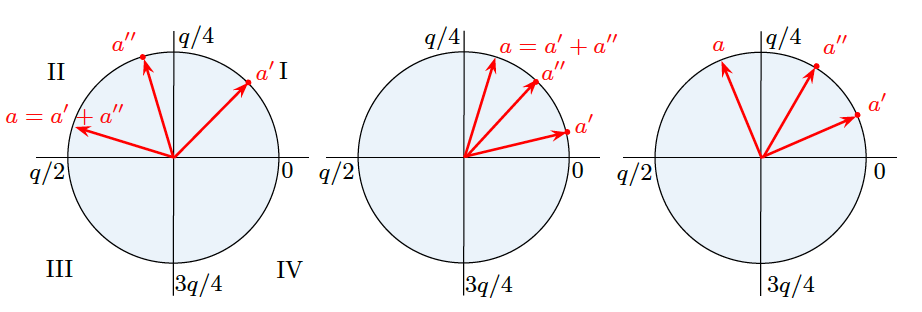
\includegraphics[width=\textwidth]{maskedDecoder_1.png}
	\caption{The basic idea of our masked decoder. The circle represents elements in \(\mathbb{Z}_q\). The first case shown allows us to conclude \(\textsc{Decode}(a)=1\), while we cannot make any guesses about the last two ones. \cite{maskedRing}}
	\label{maskedDecoder_1}
\end{figure}
Figure \ref{maskedDecoder_1} shows our example from above on the left. We can use this knowlegde to state a total of four rules, the first of whom is taken from our example:
\begin{itemize}
\item \(0 < a' < q/4\), \(q/4 < a'' < q/2\) \(\implies\) \(a \in (q/4,3q/4)\) \(\implies\) \(\textsc{Decode}(a)=1\)
\item \(q/2 < a' < 3q/4\), \(3q/4 < a'' < q\) \(\implies\) \(a \in (q/4,3q/4)\) \(\implies\) \(\textsc{Decode}(a)=1\)
\item \(q/4 < a' < q/2\), \(q/2 < a'' < 3q/4\) \(\implies\) \(a \in (0,q/4) \cup (3q/4,q)\) \(\implies\) \(\textsc{Decode}(a)=0\)
\item \(3q/4 < a' < q\), \(0 < a'' < q/4\) \(\implies\) \(a \in (0,q/4) \cup (3q/4,q)\) \(\implies\) \(\textsc{Decode}(a)=0\)
\end{itemize}
With swapping \(a'\) and \(a''\) in the above rules, one can obtain another four rules. From the rules it follows, that we only need to know the quadrant of each \(a'\) an \(a''\) to infer the output of \(\textsc{Decode}(a)\). However, this does not work for all cases, as Figure \ref{maskedDecoder_1} shows. We can actually only apply those rules in half of the possible cases.\\
So, what happens if our \((a', a'')\) does not match any rule? We simply need to refresh the splitting by computing \(a' = a' + \Delta_1\) and \(a'' = a'' - \Delta_1\) with \(\Delta_i \in \mathbb{Z}_q\). From \((a' + \Delta_1) + (a'' - \Delta_1) = a' + a'' = a\) it follow, that \(a\) stays unchanged by that refresh. Now that we have a fresh pair \((a',a'')\), we can again try to apply our rules from above. This process can be repeated until all shares have been decoded. Note, that a new \(\Delta_i\) should be choosen for each iteration. About half of the \(a',a''\) are decoded per iteration, so that the amount of decoded shares rises exponentially with the number of iterations. The authors of \cite{maskedRing} propose a number of \(N = 16\) iterations for a satisfactory result.
\begin{figure}[H]
	\centering
	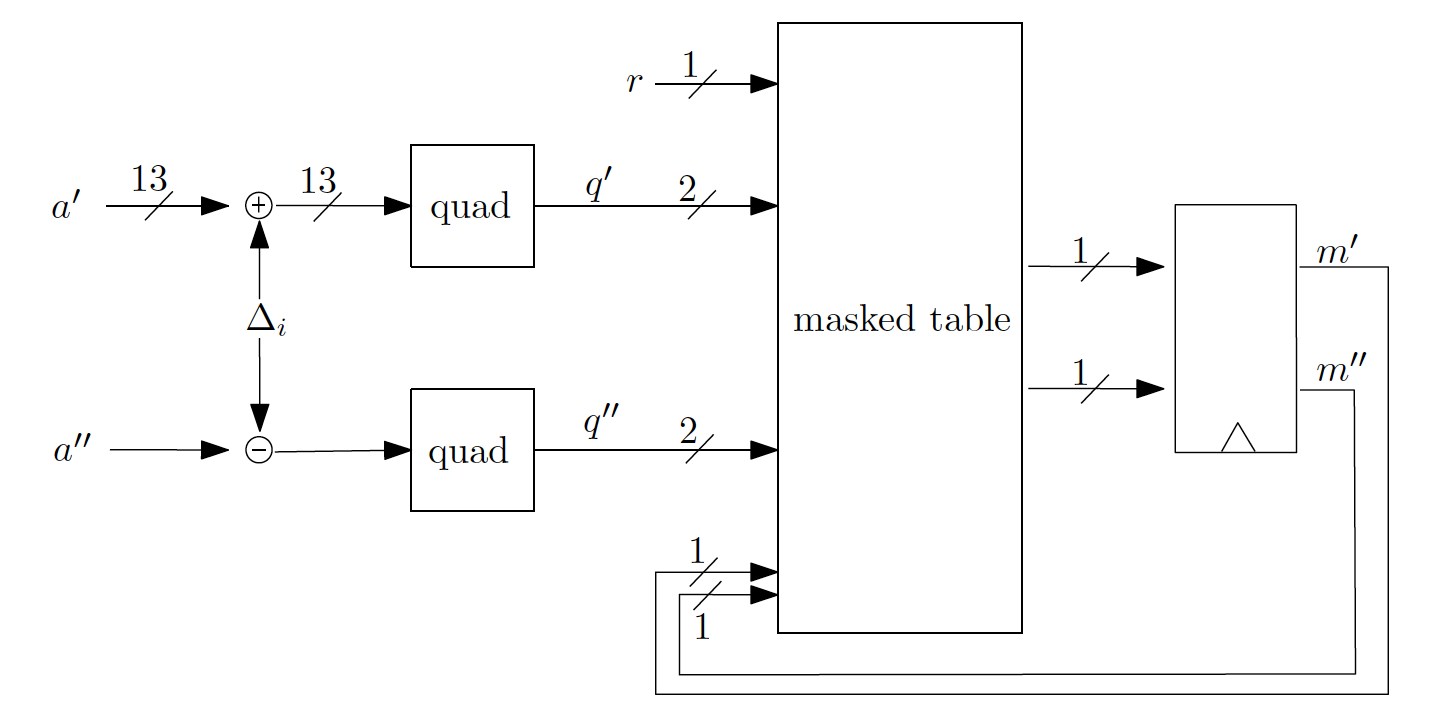
\includegraphics[width=0.7\textwidth]{maskedDecoder_2.png}
	\caption{Hardware implementation of the masked decoder. \cite{maskedRing}}
	\label{maskedDecoder_2}
\end{figure}
A possible hardware implementation of such a masked decoder is shown in Figure \ref{maskedDecoder_2}. The refreshing step is depicted on the left, using a different \(\Delta_i\) in each iteration. The quadrant function used in the next step simply takes a refreshed share \(a'\) or \(a''\) as an input and outputs two bits depending on the quadrant that the share belongs to. Next, a masked table is used to check the two bits against the rules we described above. Finally, the masked table function returns two one bit shares of the decoded message \(\textit{m}\). In our implementation the masked takes additional inputs, like a random bit \(r\) and the output of the last iteration \((m_{i-1}',m_{i-1}'')\). For more details on the masked table lookup, we would like to refer you to the paper of Oscar Reparaz et. al. \cite{maskedRing}.

%\subsection{Masked Table Lookup}
%Wenn noch Text fehlt, wird das hier eingefügt

\section{Evaluation}
Starting with efficiency, Reparaz et. al. showed that this implementation is at least 1.9x times better on a Virtex-2 FPGA than an unprotected high-speed elliptic curve scalar multiplier architecture introduced in \cite{Rebeiro2012}.\\
Furthermore, as both, the \textit{\ac{LPR} \ac{ring-LWE}} encryption scheme and our masked decoder, are probabilistic, there will always be a chance for errors occuring during decoding. The global error rate of decoding rises significantly when using our masked decoder instead of a deterministic decoder. To offset this effect, we can adapt the number of iterations for the masked decoder. While for \(N=3\) iterations the global error rate is about \(49\) times larger than when using a deterministic decoder, \(N=16\) iterations yield a global error rate that is almost identical with the one of a deterministic decoder. Further improvement could be achieved by increasing the number of iterations again, but this would lead to a significantly higher cycly count and thus to a much more inefficient implementation.
\\For our evaluation in terms of side-channel attack soundness, we assume the attacker knows the details of our implementation and is aware of the rest of the key while guessing a subkey. Our evaluation will follow three steps: First, we perform a first-order key recovery attack with our source of randomness (\textit{\acs{PRNG}}) turned off. This attack will be successful, showing that our setting is correct. In the second step, we will turn on the PRNG and repeat the same attack, but it should not be successful in this case. Finally, we perform a second-order attack to confirm the correctness of the first two steps.
\begin{figure}[H]
	\centering
	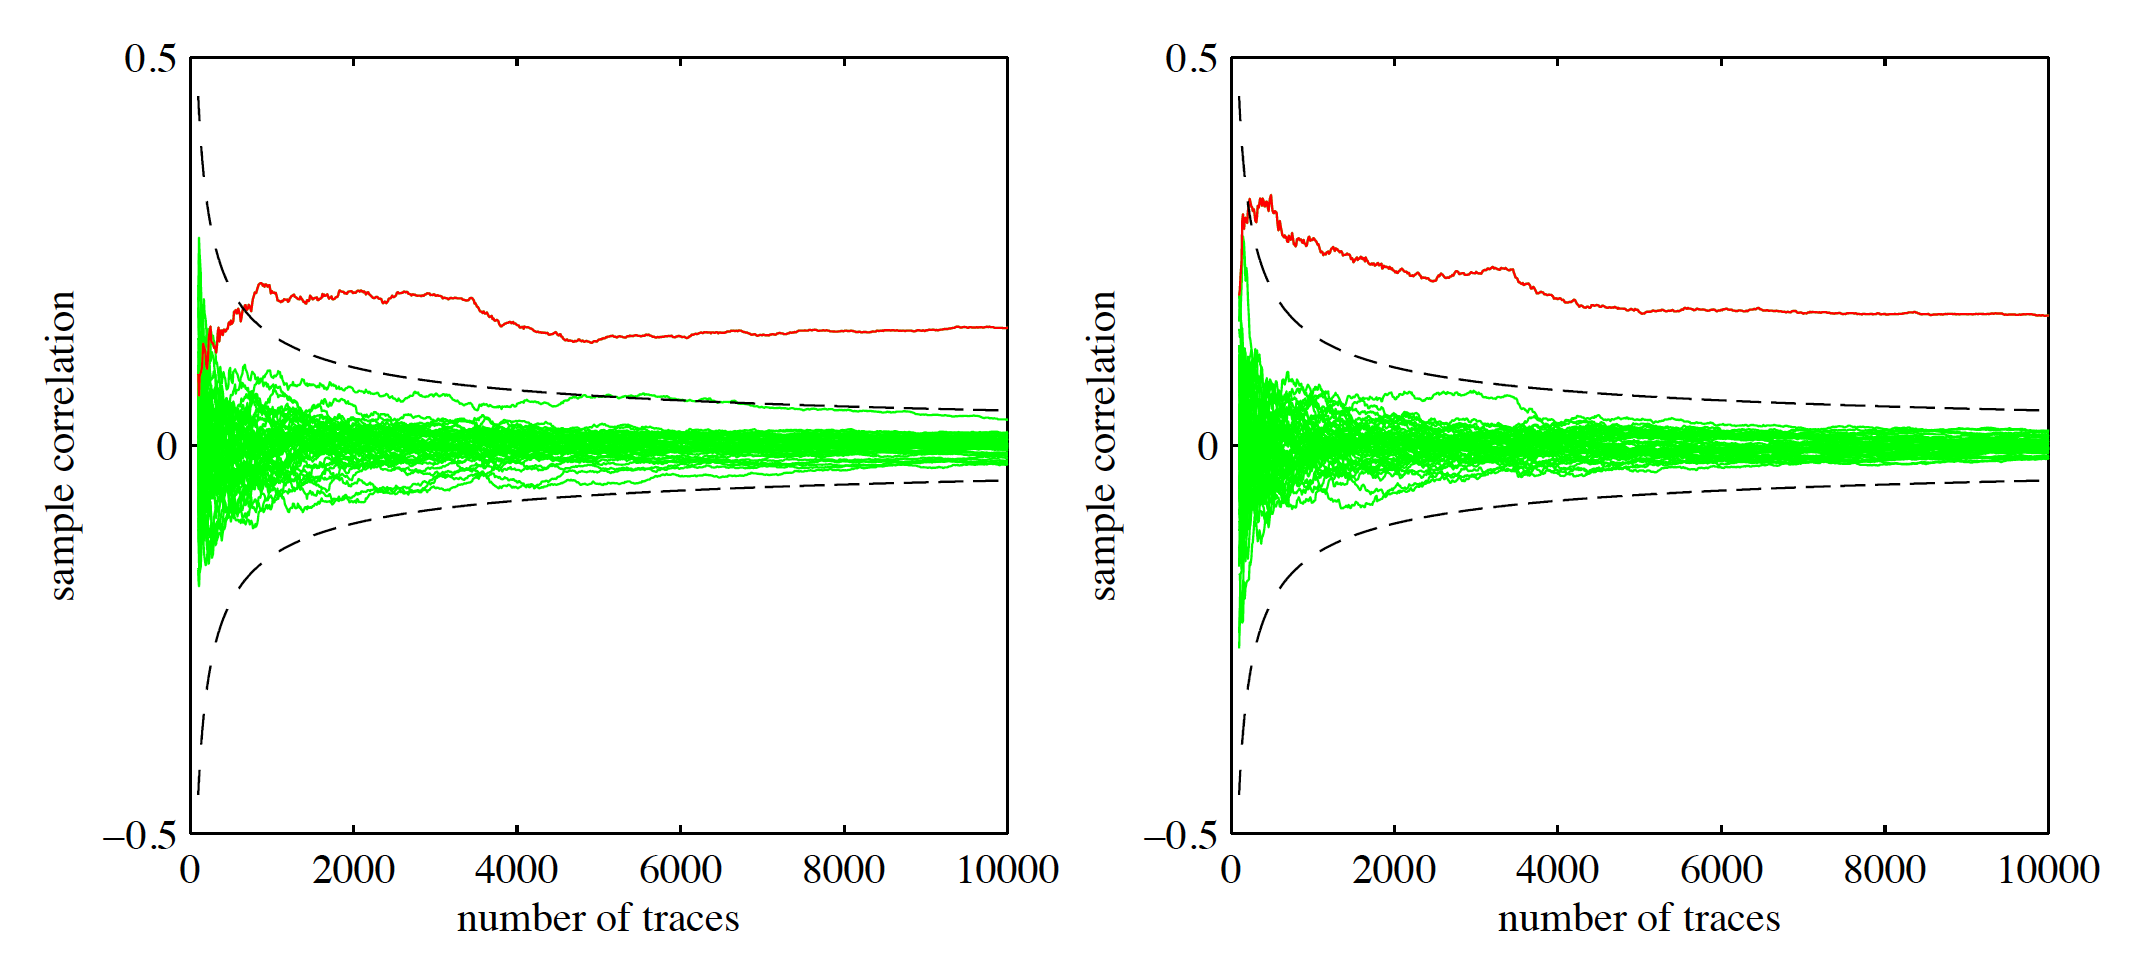
\includegraphics[width=0.7\textwidth]{dpa_1.png}
	\caption{\textit{\acs{PRNG}} is turned off. Graph shows the correlation coefficient increasing with the number of traces for the intermediates \(a'_0\) (left) and \(a''_0\) (right). The correct subkey is shown in red, all other guesses in green. \cite{maskedRing}}
	\label{dpa_1}
\end{figure}
For each of those steps, four different points that cover all relevant steps of the algorithm have been tested. The targets are \(a'_0\), \(a''_0\), the first input to the masked decoder and the first output bit. Pearson's correlation coefficient has been used to compare our guesses with real measurements \cite{Brier2004}.
\\\textbf{\textit{\acs{PRNG}} off:} When the \textit{\ac{PRNG}} is turned off, sharing of \(\textbf{s}\) in \(\textbf{s}'\) and \(\textbf{s}''\) is deterministic. This translates to the masking being turned off. Figure \ref{dpa_1} shows the correlation coefficient evolving with the number of traces. The attack seems to be successful starting at about a hundred traces.
\begin{figure}[H]
	\centering
	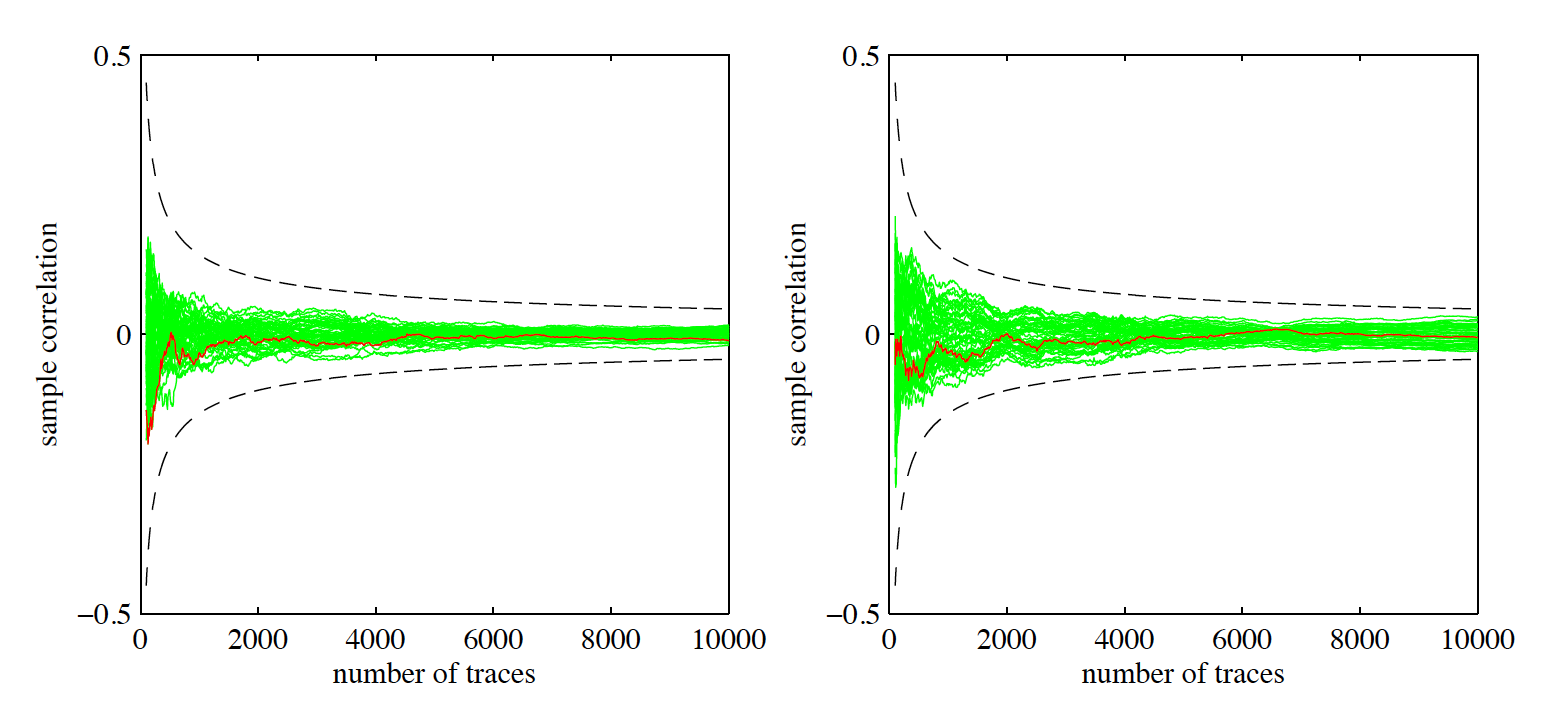
\includegraphics[width=0.7\textwidth]{dpa_2.png}
	\caption{Same as Figure \ref{dpa_1}, but with the \textit{\acs{PRNG}} turned on. It is no longer possible to identify the correct subkey within all guesses, meaning that the masking is successful. \cite{maskedRing}}
	\label{dpa_2}
\end{figure}
\textbf{\acs{PRNG} on:} When the \textit{\acs{PRNG}} is turned on, the masking is effective. As we can see in Figure \ref{dpa_2}, the correct subkey can no longer be distinguished from all the other guesses, not even with an enormous amount of traces. This is what an attacker would see when conducting an first-order \textit{\ac{DPA}} on our masking scheme.
\begin{figure}[H]
	\centering
	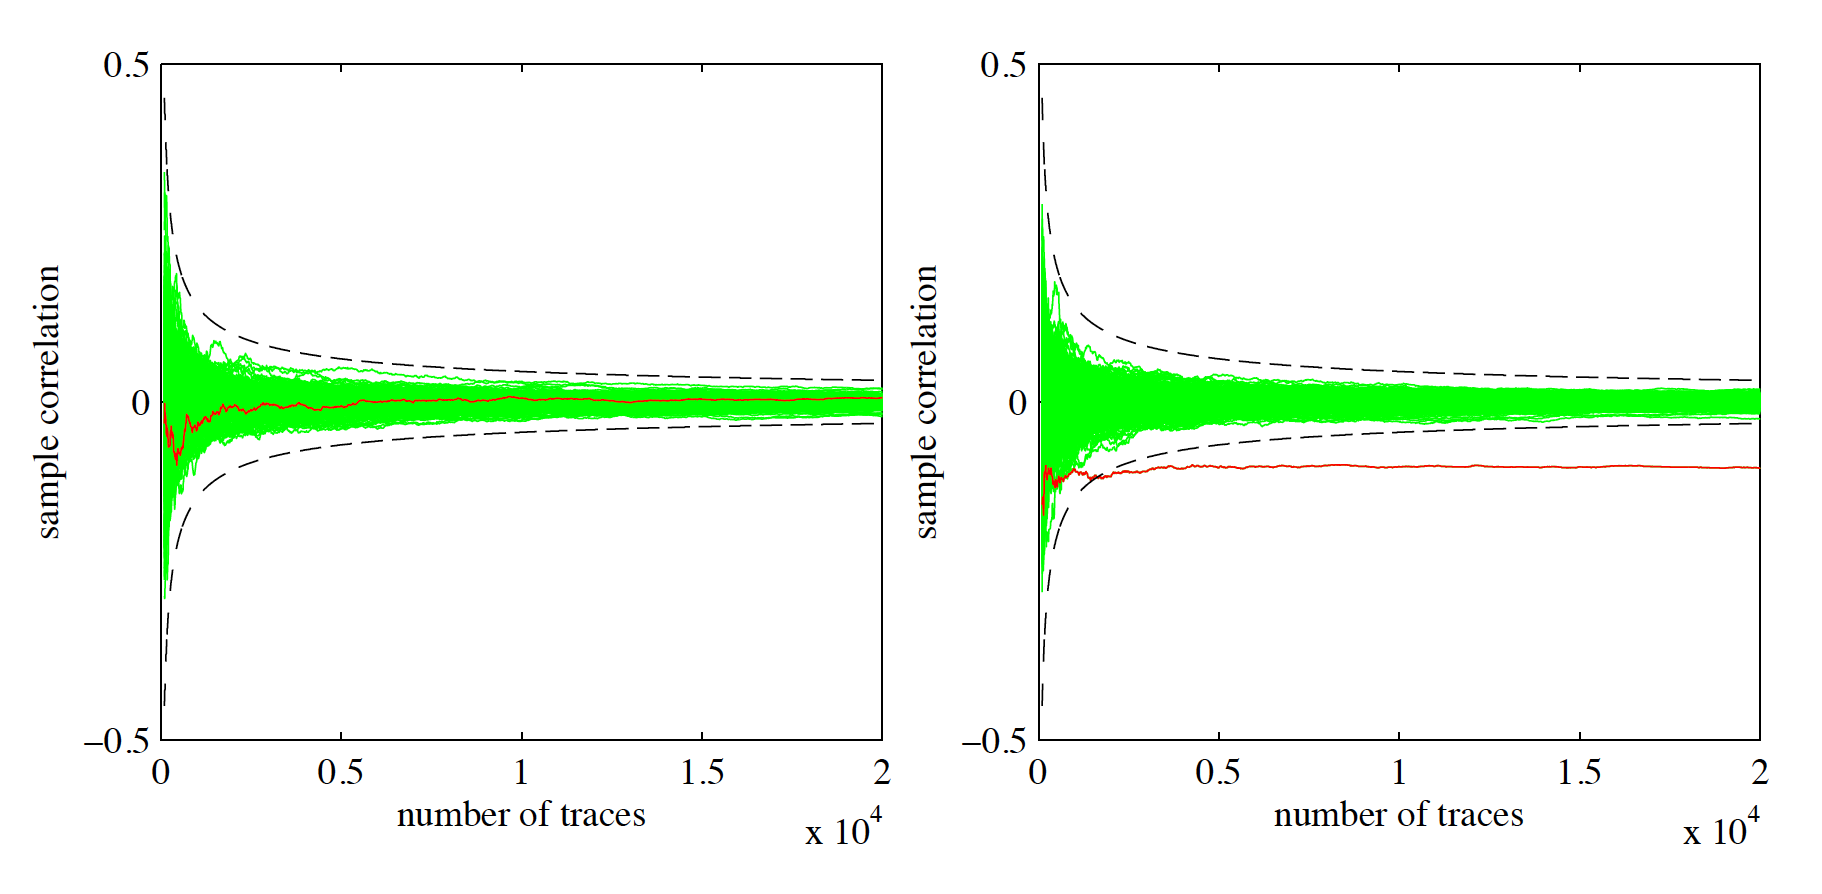
\includegraphics[width=0.7\textwidth]{dpa_3.png}
	\caption{On the left is the correlation for an increasing number of traces of a first-order attack with masking turned on. On the right we can see a successful second-order attack on our decoding scheme with masking turned on. \cite{maskedRing}}
	\label{dpa_3}
\end{figure}
\textbf{Second-Order Attack:} To confirm that we have used a sufficient number of traces in the first two steps, we perform a second-order attack on our masking scheme. In Figure \ref{dpa_3} we can see, that the second-order attack starts to be successful at around 2000 traces. From this we conclude, that we carried out the first-order attack on the activated masking scheme correctly, as we are already successful with 2000 traces. We stress that an attacker would need a significantly higher number of traces and computations in reality, as we used a pretty friendly setting for our scenario.
%
% Sample conclusion of your thesis
%

\chapter{Additively Homomorphic ring-LWE Masking}
Less than a year after \cite{maskedRing} (which has been described in the last Section) was published, Reparaz et. al. published a follow-up paper \cite{Reparaz2016} introducing a much easier approach for the masking of the \ac{ring-LWE} encryption scheme.\\
In the following, the approach of said paper will be introduced and evaluated in terms of efficiency and side-channel attack resistance. In our description we again focus on the \ac{LPR} scheme, though the techniques are also applicable for other \ac{ring-LWE} encryption schemes.

\section{Implementation}
For \ac{ring-LWE} masking, we make use of the fact that the \ac{LPR} encryption scheme is additively homomorphic. Thus for given ciphertexts \((\textbf{c}_1, \textbf{c}_2)\) and \((\textbf{c}'_1, \textbf{c}'_2)\), which are the encryption of two messages \(\textbf{m}\) and \(\textbf{m}'\) with \(m_i, m'_i \in \{0,1\}\) using the same public key \(\textbf{p}\), it follows that \((\textbf{c}_1+\textbf{c}'_1, \textbf{c}_2+\textbf{c}'_2)\) is the encryption of \(\textbf{m} \oplus \textbf{m}'\). As a consequence we can write down the following equation:
\begin{equation}
	decryption(\textbf{c}_1,\textbf{c}_2) \oplus decryption(\textbf{c}'_1,\textbf{c}'_2) = decryption(\textbf{c}_1 + \textbf{c}'_1,\textbf{c}_2 + \textbf{c}'_2)
\end{equation}
Now, we want to make use of the prperty of additive homomorphism for our masking scheme. This, again, focuses on the decryption function, as this is the part of the encryption scheme, where the secret key is used, which makes it a prime target for attackers.\\
To randomize the decryption of \((\textbf{c}_1, \textbf{c}_2)\), we need to follow three simple steps:
\begin{enumerate}
\item Generate a random message \(\textbf{m}'\) unknown to the adversary
\item Encrypt \(\textbf{m}'\) to \((\textbf{c}'_1, \textbf{c}'_2)\)
\item Decrypt \((\textbf{c}_1+\textbf{c}'_1, \textbf{c}_2+\textbf{c}'_2)\) to receive \(\textbf{m} \oplus \textbf{m}'\)
\end{enumerate}
The masked message returned by this approach is \((\textbf{m}', \textbf{m} \oplus \textbf{m}')\), such that \(\textbf{m} = (\textbf{m} \oplus \textbf{m}') \oplus \textbf{m}'\).\\
The advantage of this approach is, that no masked decoder is needed. For decoding, an unprotected decoder might be used without leaking any useful information for an attacker.

\section{Evaluation}
%
% Sample conclusion of your thesis
%

\chapter{Flush+Reload Cache Attack on Bliss}
\label{bliss}

\section{Gaussian Sampling} %Eventuell zur Theorie
The Gaussian Sampler is an important part for the security of many lattice based cryptosystems, because it is used to generate important values. This task is essential for the security of the cipher or signature, so the sampler is likely target of an attacker. There are many papers dealing with various ways of discrete gaussian sampling such as \cite{cryptoeprint:2010:088}, but in this chapter we will introduce the two different Gaussian Samplers and side channel attacks as described in \cite{cryptoeprint:2016:300}.
\subsection{CDT Sampling}
Using the cumulative distribution function in the sampler, we build a large table, in which we approximate the probabilities $p_y=\mathbb{P}[x \le y| x \leftarrow D_\sigma ]$ with $\lambda$ Bits of precision. At sampling time, we generate a uniformly random $r \in [0,1)$ and perform a binary search in the table to locate $y \in [-r\sigma, r\sigma]$, so $r \in [p_{y-1}, p_y)$. If restricted to the non-negative part $[0, r\sigma]$, the probabilities are $p^*_y = \mathbb{P}[|x| \le y| x \leftarrow D_\sigma]$, sampling is still $r \in [0,1)$, but $y \in [0, r \sigma]$ is located. 

The binary search in this sampling method can take some time, so one can speed it up by using an additional \textit{guide table I}. This table stores for example 256 entries consisting of intervals $I[u] = (a_u, b_u), u \in \{0,...255\}$ such that $p^*_{a_{u}} \le u/256$ and $p^*_{b_{u}} \ge (u+1)/256$. At sampling time, the first byte of $r$ is then used to select the corresponding $I[u]$, which leads to a smaller interval to binary search. $r$ is effectively picked byte-by-byte using the guide table approach. Algorithm \ref{algcdtwtable} summarizes the guide table approach.
 \begin{algorithm}
 	\caption{CDT Sampling With Guide Table}
 	\label{algcdtwtable}
 	\begin{algorithmic}[1]
 		\Require{ Big table $T[y]$ containing values $p^*_y$ of the cumulative distribution function of the discrete Gaussian distribution (using only non-negative values), omitting the first byte. Samll table $I$  consisting of the 256 intervals.}
 		\Ensure{Value $y \in [-r\sigma, r\sigma]$, sampled with probability according to $D_\sigma$}
 		\State{pick a random byte $r$}
 		\State{Let $(I_{min}, I_{max}) = (a_r, b_r)$ be the left and right bounds of interval $I[r]$}
 		\If{$I_{max}-I_{min} = 1$}
	 		\State{generate a random sign bit $b \in \{0,1\}$}
	 		\State
	 		\Return {$y=(-1)^bI_{min}$}
	 	\EndIf
	 	\State{Let $i=1$ denote the index of the byte to look at}
	 	\State{Pick a new random byte r}
	 	\While{$1$}
			\State{$I_z = \lfloor \frac{I_{min}+I_{max}}{2}\rfloor$} 
			\If{$r > (i$th byte of $T[I_z])$}
				\State{$I_{min} = I_z$}
			\ElsIf{$r < (i$th byte of $T[I_z])$}
				\State{$I_{max} = I_z$}
			\ElsIf{$I_{max}-I_{min} = 1$}
				\State{generate a random sign bit $b \in \{0,1\}$}
				\State
				\Return{$y=(-1)^bI_{min}$}
				\Else
				\State{increase $i$ by $1$}
				\State{pick new random byte r}
			\EndIf	
		\EndWhile
 	\end{algorithmic}
 \end{algorithm}
\subsection{Rejection Sampling}
Rejection Sampling basically accepts a sampled uniformly random integer $y \in [-r\sigma, r\sigma]$ with probability $p_\sigma(y)/p_\sigma(\mathbb{Z})$. This is done by sampling a uniformly random value $r \in [0,1)$ and accepting the unformly random $y$ if $r \le p_\sigma(y)$. This procedure can be quite expensive, because $p_\sigma(y)$ has to be calculated to a high precision and even then the rejection rate may be quite high.

The authers of \cite{bliss} which introduced BLISS proposed a more efficient rejection sampling algorithm, which will be used in the following chapters.%kann man das so schreiben

This algorithm reduces the amount of rejected samples significantly. It begins with sampling a value $x$ according to the binary discrete Gaussian distribution $D_{\sigma 	_{2}}$ with $\sigma _2 = \frac{1}{2 ln 2}$. Uniformly random bits can be used to do this efficiently. $y = Kx + z, z \in \{0,...,K-1\}$ is then uniformly random sampled and $K = \lfloor\frac{\sigma}{\sigma _2} + 1\rfloor$ is distributed according to the targeted discrete Gaussian distribution $D_\sigma$ by rejecting when $b = \exp (−z(z + 2Kx)/(2σ^2)) = 0$ holds.

This last step still requires some computing because of the exponential value $b$, but the authors provided a more efficiant algorithm for this, too. %algorithmen einfügen
 \begin{algorithm}
 	\caption{Sampling from $D^+_{K_{\sigma}}$ for $K\in\mathbb{Z}$}
 	\label{algrjt1}
 	\begin{algorithmic}[1]
 		\Require{Target standard deviation $\sigma$, integer $K = \lfloor \frac{\sigma}{\sigma_2} +1$, where $\sigma_2 = \frac{1}{2ln2}$}
 		\Ensure{Integer $y \in \mathbb{Z}^+$ according to $D^+_{K_{\sigma_{2}}}$}
 		\State{sample $ x \in \mathbb{Z}$ according to $D^+_{K_{\sigma_2}}$}
 		\State{sample $z \in \mathbb{Z}$ unformly in $\{0,...K-1\}$}
 		\State $y \leftarrow Kx + z$
 		\State sample b with probability $exp(-z(z+2Kx)/(2\sigma^2))$
 		\If{$b=0$}
	 		\State
	 		\Return{$y$}
 		\EndIf	
 	\end{algorithmic}
 \end{algorithm}
 \begin{algorithm}
 	\caption{Sampling from $D_{K_{\sigma}}$}
 	\label{algrjt2}
 	\begin{algorithmic}[1]
 		\Ensure{An integer $y \in \mathbb{Z}$ according to $D_{K_{\sigma}}$}
 		\State Sample integer $y \leftarrow D^+_{K_{\sigma}}$ using algorithm \ref{algrjt1}
 		\If{$y = 0$}
	 		\State restart with probability $1/2$
	 	\EndIf
	 	\State generate random bit b and \Return{$(-1)^by$}
 	\end{algorithmic}
 \end{algorithm}
  \begin{algorithm}
  	\caption{Sampling a bit with probability $exp(-x/(2\sigma^2))$ for $x \in [0, 2^\ell=$}
  	\label{algrjt3}
  	\begin{algorithmic}[1]
  	 \Require{$x \in [0,2^\ell)$ an integer in binary form $x = x_{\ell-1}...x_0$. Table $ET$ with precomputed values $ET[i] = exp(-x/(2\sigma^2))$ for $0 \le i \le \ell-1$}
  	 \Ensure{A bit $b$ with probability $exp(-x/(2\sigma^2))$ of being $1$}
  	 \For{$i = \ell -1$}
	  	 \If{$x_i = 1$}
		  	 \State Sample $A_i$ with probability $ET[i]$
		  	 \If {$A_i = 0$} \Return{0}
		  	 \EndIf
		 \EndIf
	 \EndFor
	 \State
	 \Return{1}
  	\end{algorithmic}
  \end{algorithm}

\section{The FLUSH+RELOAD Cache Attack}
The attack used in \cite{cryptoeprint:2016:300} is the FLUSH+RELOAD cache attack. This attack abuses the fact, that modern CPUs feature multiple different cache levels, for example L1 cache. This is the fastest and smallest cache level and located closest to the cpu core. The next level, L2 cache, is bigger and slower than L1, L3 is even bigger and slower than L2, etc.

If the CPU has to access a memory address, it looks for the corresponding memory block in higher levels first. If the block is found, a \textit{cache hit}, the data is accessed. But in case of a \textit{cache miss}, it starts to look for the memory block on lower cache levels down to the system memory. If the corresponding block is found in lower levels, the processor \textit{evicts} a cache line in the higher memory and places the found memory line there, to speed up future access on the same memory block.

The higher access times on lower cache levels are exploited by cache timing attacks like the FLUSH+RELOAD attack. The attacker has to use the same memory as the victim to apply this kind of attack. He can monitor the state of the cache and use the timing differences to check which memory blocks are cached and which addresses were accessed by the victim. If done correctly, the attacker can deduce the cache lines of the victims table access, which limits the possible chosen values.


The FLUSH+RELOAD attack abuses the x86\_64 instruction \verb|clflush| to evict a memory block from cache, before the victim executes his algorithm. After the victim is done with his memory access, he measures the time to access the memory block again. If the victim accessed the memory block, the block will be in a fast cache level and the access time will be low. If it was not accessed, the CPU has to load the memory block from a lower cache level and the access will be much slower. The attacker then knows, if the flushed memory block was accessed or not.

\subsection{Attacking CDT Sampling}
The CDT sampling algorithm with an interval table $I$ and a table with actual values $T$ like in algorithm \ref{algcdtwtable} can leak information based on cache hits and cache misses.

A cache attack as described above can only yield the cache lines of index $u$ of the interval table and the cache line of index $I_z$ of the look-up in $T$. This leaves a range of values for $|y_i|$, additionally the sign of $y_i$is not stored in the table. But the combination of both table look-ups can yield precise information, too.
Two possible combinations of table accesses are \textit{intersection} and \textit{last-jump}. \\
The intersection cache weakness intersects knowledge about index $u$ in $I$ and the access $T[I_z]$. Sometimes values in the range of intervalls are largly not overlapping with the range of values from $T[I_z]$, so the intersection %schnittmenge?!
narrows down the possible values. If, for example, the sample $|y_i|$ has to be in the set $S_1 = \{0,1,2,3,4,5,6,7,8\}$ according to the cache line $I[u]$, but $T[I_z]$ reveals $|y_i|$ must be in $S_2 = \{8,9,10,11,12,13,14,15\}$, we can learn $|y_i| \in S_1 \cap S_2 = \{7,8\}$.\\
Another abusable weakness is called \textit{last-jump} and can be used if elements of an interval $I[u]$ are spread over two cache lines of $T$. For example interval $I[u] = {5,6,7,8,9}$ is divided over cache-lines $T_1 = \{0,1,2,3,4,5,6,7\}$ and $T_2 = \{8,9,10,11,12,13,14,15\}$. A binary search will start at the value $7$ in the always accessed cache-line $T_1$, but cache-line $T_2$ is only accessed, if $|y_i| \in \{8,9\}$.\\
\cite{cryptoeprint:2016:300} restricted the patterns even more: 
\begin{itemize}
	\item To limit the maximum possible error of $|y_i|$ to at most 1, only the weaknesses are used, in which the number of candidates for $|y_i|$ is 2.
	\item Because adjacent intervals can partially overlap, $I[u] \cap I[v] \neq 0$ for $u = v+1$, for certain parts of $I[u]$, the outcome of the sample is biased.
	The second restriction considers only cache weaknesses for which one of the two candidates is much more likely to be sampled.
	\begin{equation*}
		\mathbb{P}[|y_i| = \gamma_1 | y_i \in \{\gamma_1,\gamma_2\}\subset I[u]] \gg \mathbb{P}[|y_i| = \gamma_2 | y_i \in \{\gamma_1,\gamma_2\}\subset I[u]]	
	\end{equation*}
	Values $\gamma_1$ with $\mathbb{P}[X=\gamma_1 | X \in \{\gamma_1, \gamma_2\}\subset I[u]] = 1-\alpha$ with small $\alpha$ are wanted.
	Together with the first restriction, a matched access pattern is almost always $\gamma_1$.
	\item To learn the sign of $|y_i|$, only cache patterns with $|y_i| > \beta \cdot \mathbb{E}[\langle s,c \rangle ], \beta \ge 1$ are used. By looking at the sign of $z_i$ the sign of $y_i$ can be learned, because 
	\begin{equation*}
	sign(y_i) \neq sign(z_i) \iff \langle s,c \rangle > (y_i+z_i)	
	\end{equation*}
\end{itemize}
Choosing different values $\alpha$ and $\beta$ is flexible, but might lead to no matching access patterns or let other parts fail. The paper described $\alpha \le 0.1$ had at least one usable cache access pattern for every parameter set. $\beta$ was not used in the experiments.

The attack assumes a cache access pattern reveals if $y_i \in \{\gamma_1, \gamma_2\}$ for $i = 0,...,n-1$ of polynomial $y$ and $\mathbb{P}[y_i = \gamma_1] = 1- \alpha$ with small $\alpha$. \\
The victim then has to generate $N$ signatures $(z_j, c_j), j= 1,...,N$, which are collected by the attacker and the corresponding cache information for the noise polynomial $y_i$. When a cache weakness is found, the attacker has to solve the equation 
\begin{equation*}
	z_{ji} = y_{ji} + (-1)^{b_j}\langle s,c_ji \rangle
\end{equation*}
Unknown values are $b_j$ and $s$. Because of restrictions above, if $z_{ji = \gamma_1}$, the attacker adds $\xi_k = c_{ji}$ to a list of good vectors. With enough vectors $\xi_k = c_{ji}; 0 \le i \le n-1, 1 \le j \le N, 1 \le k \le n$ the matrix $L \in \{-1,0,1\}^{n \times n}$ can be formed. The column vectors $\xi_k$ satisfy $sL = v$, where $v$ is a unknown, but short, vector with norm about $\sqrt{\alpha n}$ in the lattice spanned by the rows of $L$. A lattice reduction algorithm, like LLL, can search for $v$ and output a uni-modular matrix $U$ with $UL = L'$. Every row of $U$ (or its rotations) is tested if it is a candidate for $s=f$ by checking against the public key.

Because this last step is not always successful, not only $n$ but $m>n$ vectors $\xi_k$ are collected and a random subset forms the input for LLL.

\begin{algorithm}
	\caption{Cache attack on BLISS with CDT Sampling}
	\label{algcdtattack}
	\begin{algorithmic}[1]
		\Require{Access to cache memory of a victim with a key-pair $(A,S)$. BLISS input parameters $n, \sigma, q, \kappa$ with $\kappa <K$. Access to signature polynomials $(z_1, z_2^\dagger, c)$ produced using $S$. Victim uses CDT sampling with tables $T, I$ for noise polynomial $y$. Cache weakness that allows to determine if coefficient $y_i \in \{\gamma_1,\gamma_2\}$ of $y$, and when this is the case, the value of $y_i$, is biased towards $\gamma_1$}
		\Ensure{Secret key $S$}
		\State{Let $k = 0$ be the number of vectors gained so far and let $M=[]$ be an empty list of vectors}
		\While{$k<m$ (m vectors before randomising LLL)}
		\State{Collect signature $(z_1, z_2^\dagger, c)$ together with cache information for each coefficient $y_i$ of noise polynomial $y$}
		\For{$i=1,...,n$}
		\If{$y_i \in \{\gamma_1, \gamma_2\}$ (according to cache information), and $z_{1i} = \gamma_1$}
		\State{add vector $\xi_k = c_i$ as a column to M and set $k = k + 1$}
		\EndIf
		\EndFor
		\EndWhile
		\While{1}
			\State Choose random subset of n vectors from $M$ and construct matrix $L$ whose columns are those vectors from $M$
			\State Perform LLL basis reduction on L to get $UL = L'$, where $U$ is a uni-modular transformation matrix and $L'$ is LLL reduced.
			\ForAll{$J=1,...,n$}
				\State check if row $u_j$ of U has the same distribution as f and if $(a_1/2)\cdot u_j \bmod 2q$ has the same distribution as $2g+1$. Lastly verify if $a_1 \cdot u_j + a_2 \cdot (a_2/2)\cdot u_j \equiv q \bmod 2q$
				\State
				\Return $S = (u_j, (a_1/2)\cdot u_j \bmod 2q)$ if this is the case
			\EndFor
		\EndWhile
	\end{algorithmic}
\end{algorithm} 
\subsection{Attacking Rejection Sampling} \label{rejection}
When rejection sampling is used in the BLISS signature scheme, the side channel has to decide, if there was a table acces in the $ET$ table. The attack exploits the small size of the $ET$ table, which leaks very precise information about the sampling process.

Depending on the bit $i$ of input $x$, $ET[i]$ is accessed, if $x = 0$, no table look-up is performed. If the attacker detects this, he knows $z=0$ is the sampled value in step 2 in algorithm \ref{algrjt1}. In this case the attacker can assume $y \in \{0, \pm K, \pm 2K,...\}$ for usable cache access patterns.

So the attacker knows the coefficients $y_i \in \{0, \pm K, \pm 2K,...\}, i \in \{0,...,n-1\}$ of the noise polynomial y. Because anyone can check if $max|\langle s,c \rangle |\le \kappa < K$ with the public parameters, $y_i$ can be determined completely with the signature vector $z$. With $N$ more signatures $(z_j, c_j), j =1,...,N$, the attacker can search for  $y_{ji} \in \{0, \pm K, \pm 2K,...\}$ ($y_{ji}$ means the ith coefficient of $y_j$). If the attacker additionally sees, that $z_{ji} = y_{ji}$, he knows $\langle s, c_{ji} \rangle = 0$. Such vector is a \textit{good vector} for use in the attack and $\zeta _k = c_{ji}$ is saved for later (some known $y_{ji}$ will be discarded, if they dont satisfy the necessary requirements). With $n$ of these vectors $\xi _k = c_{ji}; 0 \le i \le n-1, 1 \le j \le N, 1\le k \le n$ a matrix $L \in \{-1,0,1\}^{nxn}$ can be formed. The column vectors $\xi_k$ satisfy $sL = 0$ (0 is the all-zero vector) and most likely the only dependency of $\xi_k$ is introduced by s, so s is the only kernel vector. There is no need to randomize this process, because the all-zero vector is used.

\begin{algorithm}
	\caption{Cache attack on BLISS with Rejection Sampling}
	\label{algrctattack}
	\begin{algorithmic}[1]
		\Require{Access to cache memory of a victim with a key-pair $(A,S)$. BLISS input parameters $n, \sigma, q, \kappa$ with $\kappa <K$. Access to signatures $(z_1, z_2^\dagger, c)$ produced using $S$. Victim uses rejection sampling with small exponential table to sample noise polynomial y}
		\Ensure{Secret key $S$}
		\State{Let $k = 0$ be the number of vectors gained so far and let $M=[]$ be an empty list of vectors}
		\While{$k<n$}
			\State{Collect signature $(z_1, z_2^\dagger, c)$ together with cache information for each coefficient $y_i$ of polynomial $y$}
			\For{$i=1,...,n$}
				\If{$y_i \in \{0, \pm K, \pm 2K, ...\}$ (according to cache information), and $z_{1i} = y_i$}
				\State{add coefficient vector $\xi_k = c_i$ as a column to M and set $k = k + 1$}
				\EndIf
			\EndFor
		\EndWhile
		\State{Form a matrix M from the columns in $M$. Calculate kernel space of M. This gives a matrix $U \in \mathbb{Z}^{\ell \times n}$ such that $UM = 0$ where $0$ is the all-zero matrix.}
		\For{$j = 1,...,\ell$ (assume $\ell = 1$)}
			\State{check if row $u_j$ of U has the same distribution as $f$ and if $(a_1/2)\cdot u_j \bmod 2q$ has the same distribution as $2g+1$. Lastly verify if $a_1\cdot u_j + a_2\cdot(a_2/2)\cdot u_j \equiv q \bmod 2q$}
			\State{}
		\Return{$S = (u_j, (a_1/2)\cdot u_j \bmod 2q)$ if this is the case}
		\EndFor
		\State{Remove a random entry from M, put $k = k - 1$, goto step 2}
	\end{algorithmic}
\end{algorithm}   

\newpage
\section{Attacking Sampling Algorithms with a Perfect Side Channel}
The paper \cite{cryptoeprint:2016:300} provided experimental results for a perfect side-channel attack using the procedure explained. This requires the attacker to get every cache line of every table look-up while computing $y$ in CDT and rejection sampling algorithms. The victim is assumed to sign random messages and the signatures are collected by the attacker. Cache lines are 64 byte and each element is 8 byte. 
To fulfill this requirements, the authors of \cite{cryptoeprint:2016:300} modified the \textit{research oriented} C++ implementation published by the BLISS authors \cite{blisshp}. Tests were performed on a 4.1 GHz AMD FX-8350 Eight-Core CPU. NTL was used for LLL reductions and kernel calculations.
\subsection{Perfect Side Channel Attack on CDT Sampling}
A perfect side channel yields the attacker the values $\lfloor u/8 \rfloor$ and $\lfloor I_z/8 \rfloor$ of the table accesses for $I[u]$ and $T[I_z]$, the full cache line for a specific value. 

Because not every cache line contains a intersection or last-jump weakness, a one-time brute force search over the look-up tables reveals cache lines, which are exploitable, by analyzing the structure and applying the biased restriction $\alpha \le 0.1$

For each BLISS parameter set at least one usable cache weakness can be found, which can be abused. 
The attacker then collects $m$ coefficient vectors $c_j$ and runs LLL up to $t = 2(m-n)+1$ times searching for s. A bigger value $t$ is not likely to have better success probabilities, because the randomly constructed lattices have overlapping base vectors, so the authors of the paper considered a experiment failed after this number of tries. Each experiment (with different parameters and different sizes of $m$) was performed 1000 times to measure the success probability $p_{successs}$, the average number of required signatures $\bar{N}$ to get $m$ usable challenges and the average length of $v$, if one was found.
The expected number of needed signatures is:
\begin{equation*}
\mathbb{E}[N] = \frac{m}{n \cdot \mathbb{P}[CP] \cdot \mathbb{P}[\langle s_q, c \rangle = 0]}
\end{equation*}
where the event CP means a usable cache access pattern for a coordinate of $y$.

\begin{table}[ht!]
	\centering
	
	\begin{tabular}{|l|l|l|l|l|l|l|} 	
		Parameter Set & m & $p_{success}$& $||v||^2_2$&$\bar{N}$&$\mathbb{E}[N]$&Offline Time\\\hline
		\multirow{6}{22mm}{BLISS-0 $n = 256$\\$\sigma=100$\\$ \kappa=12$} & 256 & 0.690 &10 &2537 & 2518 &1.9s\\
		& 257& 0.841 & 10 & 2547 & 2528 & 2.9s\\
		&258&0.886&10&2565&2538&3.5s\\
		&259&0.903&10&2671&2548&4.0s\\
		&260&0.943&10&2580&2558&4.5s\\
		&261&0.943&10&2596&2568&4.6s
 \\\hline
		\multirow{6}{22mm}{BLISS-I $n = 512$\\$\sigma=215$\\$ \kappa=23$} & 512 & 0.655 &29 &441 & 450 &37.6s\\
		& 513& 0.809 & 29 & 442 & 451 & 60.0s\\
		&514&0.881&29&442&452&71.3s\\
		&515&0.925&29&443&453&73.9s\\
		&516&0.950&29&446&454&81.3s\\
		&517&0.961&29&446&455&85.8s
		\\\hline
		\multirow{6}{22mm}{BLISS-II $n = 512$\\$\sigma=107$\\$ \kappa=23$} & 512 & 0.478 &33 &2021 & 2020 &37.5s\\
		&513&0.675 &34&2023&2024&72.1s\\
		&514&0.772&34&2030&2028&95.6s\\
		&515&0.818&35&2033&2032&110.4s\\
		&516&0.870&35&2033&2036&117.5s\\
		&517&0.897&35&2041&2040&122.0s
		\\\hline
		\multirow{6}{22mm}{BLISS-III $n = 512$\\$\sigma=250$\\$ \kappa=30$} 
		&512&0.855&23&945&930&42.2s\\
		&513&0.950&23&946&932&51.6s\\
		&514&0.975&23&951&934&55.9s\\
		&515&0.987&24&954&935&55.9s\\
		&516&0.987&24&952&937&55.8s\\
		&517&0.996&24&957&939&54.4s
		\\\hline
		\multirow{6}{22mm}{BLISS-IV $n = 512$\\$\sigma=271$\\$ \kappa=39$} 
		&512&0.617&35&1206&1189&46.2s\\
		&513&0.817&36&1209&1191&75.3s\\
		&514&0.885&36&1211&1194&88.4s\\
		&515&0.932&36&1215&1196&93.7s\\
		&516&0.947&36&1216&1198&102.4s\\
		&517&0.955&36&1217&1201&104.4s
	\end{tabular}
	\caption{Experimental results of an attack on BLISS with CDT sampling using a perfect side channel and various parameter sets}
	\label{tab:cdtperfect}
\end{table}
We can see from the results in table \ref{tab:cdtperfect}, that the average number of signatures $\bar{N}$ needed to collect m usable columns depends more on the paramter $\sigma$ and not much on $n$, because the number of usable cache weaknesses varies with that value QUELLE. The experimental results show a much better succes probabilty $p_{success}$ for a small increase of $m$, so an attacker can reach probabilities close to $1.0$, if e simply collects enough usable signatures (\cite{cryptoeprint:2016:300} suggests picking $m \simeq 2n$). 


\newpage
\subsection{Perfect Side Channel Attack on Rejection Sampling}
The perfect side channel tells the attacker, if there was an table look-up in the table $ET$. The attack explained  in section \ref{rejection} can be applied and requires $m = n$ challenges $c_i$ for the kernel calculation, because no randomization is needed. By checking the cache lines of the small part of the table, the attacker can learn if any element has been accessed in $ET$. Only 100 experiments were performed  in \cite{cryptoeprint:2016:300}, because for all parameter sets $p_{success} = 1.0$ holds.

The expected numbers of signatures needed is:
\begin{equation*}
	\mathbb{E}[N] = ((\frac{1}{p_\sigma(\mathbb{Z})}\sum_{x=-r\sigma}^{r\sigma}p_\sigma(xK))*\mathbb{P}[\langle s_1,c \rangle = 0])^{-1}	
\end{equation*}
with $K= \lfloor \frac{\sigma}{\sigma_2}+1\rfloor$ and tail-cut $r\ge 1$. The average number $\bar{N}$ of required signatures is heavily dependent on the value $\sigma$, because $xK$ is more likely to be sampled for small $\sigma$. 
\begin{table}[h!]
	\centering
	
\begin{tabular}{|l|l|l|l|l|l|} 	
	Parameter Set & m & $p_{success}$&$\bar{N}$&$\mathbb{E}[N]$&Offline Time\\\hline
	BLISS-0 & 256 & 1.0 &1105 & 1102 &0.8s\\
	BLISS-I&512&1.0&1671 & 1694 & 14.7s \\
	BLISS-II&512 & 1.0 & 824&839 & 14.4s\\
	BLISS-III&512 & 1.0 & 3018 & 2970 & 16.0s\\
	BLISS-IV&512 & 1.0 & 4223 & 4154 & 18.1S\\
\end{tabular}
\caption{Experimental results of an attack on BLISS with rejection sampling using a perfect side channel}
\label{tab:rejectionperfect}
\end{table}
\newpage
\section{Attacking Sampling Algorithms with a Real Side Channel}
The experiments explained above used a perfect side channel to get every memory information needed to perform the attack. In the following the proof of concept implementation using a realistic FLUSH+RELOAD attack from \cite{cryptoeprint:2016:300} will be summarized.
\subsection{Attacking CDT Sampling}
Because of various CPU optimizations, like prefetchers, real world implementations cannot assume to have perfectly aligned cache lines or that every loaded cache line was accessed. The \textit{spatial prefetcher} for example pairs two adjacent lines and loads both, if one is accessed. Because this might lead to false positives, only cache weaknesses spanning two unpaired lines can be exploited. \\
The \verb|clflush| instruction is used to flush the monitored cache lines before every $y_i$ is sampled and the access time is measured afterwards. Compared to a reference loadtime, we can determine if an access happened. For simplicity, only one observed cache weakness was monitored in the experiments.\\
Using an Intel i5-3470 processor, 50 attacks on the last-jump weakness $\{\gamma_1, \gamma_2\} = \{55,56\}$ in BLISS-I were performed an it was possible to recover the private key 46 times. To collect the recommended $m = 2n = 1024$ usable equations, on average $3438$ signatures were needed. Only 5 runs of LLL were performed, still a success rate of $92\%$ shows feasibility of the attack. This might vary with different CPUs, because of different prefetchers.
\subsection{Attacking Rejection Sampling}
Because the attack on rejection sampling only needs to know, if $ET$ was accessed at all and the spatial prefetcher, who will reload odd cache lines if the even ones are accessed, flushing all cache lines and reloading only the even ones, covers the whole table $ET$. Randomization, like in CDT, was needed in this case, because the side channel was not a perfect one and some columns $\langle s, c_i \rangle \neq 0$ in L were likely collected. So again, more than n columns were collected an LLL was used to handle the errors. 
With an Intel i7-5650U again 50 attacks against BLISS-I were performed and 3 out of 6 cache lines were monitored. The private key could be recovered 44 times, while on average 3294 signatures wre needed to collect $m = n +100 = 612$ equations. LLL was performed 5 times, similar to the CDT attack.
\section{Evaluation}
As we can see above, the Gaussian Samplers are vulnerable to side channel attacks and especially the FLUSH+RELOAD cache attack is a strong attack vector. Even in a realistic experiment it was possible to compute the private key in many cases, just by monitoring the CPU cache state before and after the signature. The number of signatures needed was not very high either. Access to the systems scheduler will even reduce this number significantly.

This leads to the conclusion, that even fast and reliable gaussian sampling algorithms should be used with care, because an attacker with some kind of access to the processor can break the cryptosystem, even without access to the signature process itself. Masking is one way to reduce the risk of being successful attacked and even choosing different values for the target discrete gaussian distribution may help to avoid such an attack. 
%
% Sample conclusion of your thesis
%

\chapter{Blinding Countermeasures}

\section{Blinding Polynomial Multiplication}

\section{Blinding Gaussian Sampling}
%
% Sample conclusion of your thesis
%

\chapter{Conclusion}
This chapter gives an overview of the different attacks and countermeasures we described in this paper and summarizes the bottom line of each chapter.

We start by describing a first-order masking scheme for the decryption function of a \ac{ring-LWE} cryptoscheme. After introducing the reader to the masking approach, we present one possible implementation of the proposed masked decoder. Finally, we conclude that this scheme is efficient enough to be considered for real world applications and showed that it is indeed sound against first-order \ac{DPA}.

Furthermore, we present another masking approach for the \ac{ring-LWE} scheme, which is not as sound against first-order \ac{DPA} as the previous one, but outperforms it in terms of efficiency.

BLISS CHAPTER

Finally, we introduce the reader to two blinding countermeasures, namely blinding of polynomial multiplications and blinding of Gaussian sampling. Both of them can be used for any arbitrary lattice-based cryptosystem, but we do not give any guarantees in terms of side-channel security.




% Generate list of figures
\newpage
\listoffigures

% Generate list of tables
\newpage
\listoftables

% Generate list of algorithms
\newpage
\listofalgorithms
\clearpage

% Generate bibliography with bibtex, the bibfile here is "bibliography.bib", use alphanumerical style
\begin{appendix}
 	\bibliography{bibliography}
 	\bibliographystyle{alpha}
\end{appendix}

\end{document} 
